\documentclass[12pt,letterpaper]{article}

\PassOptionsToPackage{hyphens}{url}

\usepackage{setspace}
\doublespacing
\usepackage[]{natbib}
\bibliographystyle{apalike}
% \bibliographystyle{plainnat}

% === MARGINS ===
\addtolength{\hoffset}{-0.75in} 
\addtolength{\voffset}{-1.25in}
\addtolength{\textwidth}{1.5in} 
\addtolength{\textheight}{2.25in}

% == ENVS ==
\newenvironment{tightcenter}{%
  \setlength\topsep{0pt}
  \setlength\parskip{0pt}
  \begin{center}
}{
  \end{center}
}

% == PACKS ==
\usepackage{color,soul}
\usepackage{graphicx} % to use pngs in tex (include graphix)
\usepackage{calc} % To scale \pagewidth with \real{float}
\usepackage{pgfplots} % To draw histogram

\pgfplotsset{
  compat=1.17, 
colormap/viridis
} % request specific version of pgfplots

\usepackage{calc} % to use \real for text -> numeric
\usepackage{pgf} % to store numeric variables
\usepackage{subcaption} % to place two figures horizontally
\usepackage{caption} % to refer subfigure
\renewcommand{\thesubfigure}{(\alph{subfigure})}
\captionsetup[sub]{labelformat=simple}
\captionsetup[table]{font={stretch=1.2}}  % adjust line space in captions of TABLE and FIGURES
\captionsetup[figure]{font={stretch=1.2}}  


\usepackage{tikz}
\usetikzlibrary{automata,positioning}
\usetikzlibrary{arrows.meta, positioning, automata}
\usetikzlibrary{spy}
\usetikzlibrary{shadows}
\usetikzlibrary{arrows,positioning,shapes.geometric} % for dnn flowchart


\tikzset{
  font={\fontsize{10pt}{0}\selectfont}}
\usepackage{forest}
\tikzset{
  Decision/.style = {%
    draw,
    line width=1.4pt
  },
  Lottery/.style = {%
    draw,
    line width=1.4pt
  },
  Outcome/.style = {%
    circle,
    minimum width=3pt,
    fill,
    inner sep=0pt
  }
}
\usepackage{csquotes}
\usepackage{lipsum}
\usetikzlibrary{arrows.meta,automata,positioning} % to draw directed-weighted-graph


\usepackage{amsmath, amssymb, latexsym} % NN
\usepackage{tikz}% NN
\usetikzlibrary{decorations.pathreplacing}% NN
\usetikzlibrary{fadings}% NN


\usepackage{xltabular}
\usepackage{booktabs}

\usepackage[breakable, skins]{tcolorbox} % to add factual asepct inside a frame

\usepackage[title]{appendix}

%to prevent page and footnotes swalloen by the table


% == Checkmarks == 
\usepackage{bbding}
\usepackage{pifont}
\usepackage{wasysym}
\usepackage{amssymb}
% ================

% == BIBS ==
% \usepackage{natbib}

\usepackage{diagbox}

\usepackage[bottom]{footmisc}

\usepackage[
  hidelinks,
  pdftex, 
  bookmarksopen=true, 
  bookmarksnumbered=true,
  pdfstartview=FitH, 
  breaklinks=true, 
  urlbordercolor={0 1 0}, 
  citebordercolor={0 0 1}]
  {hyperref}

\usepackage[ruled,vlined,linesnumbered]{algorithm2e}
\SetKwFor{For}{for (}{) $\lbrace$}{$\rbrace$}

%%% Coloring the comment as blue
\newcommand\mycommfont[1]{\footnotesize\ttfamily\textcolor{blue}{#1}}
\SetCommentSty{mycommfont}

\SetKwInput{KwInput}{Input}                % Set the Input
\SetKwInput{KwOutput}{Output}   
\usepackage{algpseudocode}% http://ctan.org/pkg/algorithmicx
\usepackage{varwidth}% http://ctan.org/pkg/varwidth


\usepackage{titlesec}

\setcounter{secnumdepth}{4}

\titleformat{\paragraph}
{\normalfont\normalsize\bfseries}{\theparagraph}{1em}{}
\titlespacing*{\paragraph}
{0pt}{3.25ex plus 1ex minus .2ex}{1.5ex plus .2ex}


% == SPACES == 

% == CMMDS ==
\newcommand{\tit}{
\bf 
The Privileged Advantage: Evidence of Congressional Insider Trading
}
\newcommand\spacingset[1]{\renewcommand{\baselinestretch}
{#1}\small\normalsize}

% To draw embedding layer
\newcommand*{\xMin}{0}%
\newcommand*{\xMax}{6}%
\newcommand*{\yMin}{0}%
\newcommand*{\yMax}{9}%
% To draw conv output
\newcommand*{\xMinOut}{10}%
\newcommand*{\xMaxOut}{11}%
\newcommand*{\yMinOut}{1}%
\newcommand*{\yMaxOut}{8}%


% == VARS == 
\pgfmathsetmacro{\heatmap}{1}

\makeatletter
\setlength{\@fptop}{0pt}
\makeatother

% == START (PageCounter, Mode)
\begin{document}

\spacingset{1.25}

\setcounter{page}{0}
\vspace{-.1in}

% == TITLE (includes DraftDate)
{\title{
    \tit
  }
  \author{
    Suyeol Yun
  \thanks{Department of Political Science, MIT. Email: \href{mailto:syyun@mit.edu}{syyun@mit.edu}\\
  **The reproducible code and data can be found at the following link: \href{https://github.com/syyunn/efd}{https://github.com/syyunn/efd}.
  }
  }
  \maketitle
}

\thispagestyle{empty}
\vspace{-.1in}

\begin{abstract}
  Research on congressional investment has produced conflicting conclusions regarding whether members of Congress enjoy excess returns from their investments. In this paper, I collected all securities transaction data of US senators from 2014-2021 and found empirical evidence that excess return is not as common as the public believes. However, I address the point that a few senators were identified as enjoying outlier excess returns from their investments. I explain that excess return itself does not conclusively indicate the use of ``privileged'' or ``inside'' information, as other factors such as higher levels of general understanding of financial markets and macroeconomics could also be at play. In conclusion, further investigation and the development of proper methodologies are needed to identify the sources of excess return for those senators who have been identified as enjoying outlier excess returns. 
\spacingset{1.5} % gives a slightly more margin between abstract and introduction
\end{abstract}
\clearpage

% == INTRO ==
\section{Introduction}
\spacingset{2} % gives a slightly more margin between abstract and introduction

The investment behavior of members of Congress has long been a topic of concern among the public, the media, and scholars. The issue raises concerns about conflicts of interest, insider trading, and abuse of power, as members of Congress have access to privileged and confidential information that may provide them with an unfair advantage in the stock market. Furthermore, the use of such information for personal financial gain can be seen as a breach of public trust and may undermine the integrity of the democratic system.

In recent years, several studies have examined the investment behavior of Congressmen, including \cite{zi24}, \cite{zi11} \cite{eg13}, and \cite{eg14}. Ziobrowski's studies found that Senators and House representatives beat the market and enjoyed excess returns, while Eggers and Hainmuller's studies found the opposite. However, all of these studies were conducted using the data before the most recent legislation to regulate congressional investment, the Stock Act (2012).
Therefore, the data used in these studies are outdated, as all of them are collected before 2012. Additionally, the findings are not reproducible, as Ziobrowski refused to provide data \footnote{According to the first footnote in \cite{eg13}} and Eggers and Hainmuller lost their data as well\footnote{The authors have confirmed via email that they are unable to locate the reproducible data at this time.
}.

In response to these limitations, this paper collected data on all transaction records of Senators buying and selling securities between 2014-2021. The data was obtained from the Senate Financial Disclosure website, which provides detailed information on the securities holdings and transactions of Senators. In total, there were 25,023 transactions included in the dataset.

To assess the investment behavior of Senators, the paper computed the excess return for each life cycle of transactions, starting from the purchase of a specific ticker of securities and ending with the sale. Excess returns were computed as returns above the average risk-free federal reserve rates over those periods.

The findings of this study show that Senators do not enjoy ``wide-spread'' excess returns from their trading, which is consistent with the findings of Eggers and Hainmuller (2013). However, the study also found a few outliers who gained significant financial gains, and some of these transactions have already been exposed to the public by journalists, while others remain undisclosed.

The biggest challenge in this line of research is how to prove that Congressmen use their privileged knowledge for their stock trading. While the ``excess return'' does not necessarily imply that Congressmen use privileged knowledge, many of the famous transactions can be linked to the Congressmen's titles, committees, sponsorships, and their representation of specific states. Therefore, this research will focus on the design of proper empirical strategies to effectively track down the sources of privileged knowledge that are more closely linked to investment and that can identify instances of unethical investment behavior among Congressmen.

\section{Data}

This section describes the dataset used in this study. The data was obtained from the Senate Financial Disclosure database and an API provided by \url{Polygon.io}. This section explains the sources of the dataset, how it was collected, and the process involved in preparing the dataset for analysis.


\subsection{Sources of the dataset}

According to The Ethics in Government Act (EIGA, specifically 5 U.S.C. app. §§ 101-112) and Stop Trading on Congressional Knowledge Act (STOCK Act), senators are required to report their financial transactions to Senate and Senate maintains those information to be publicly accessible. Therefore, the list of Senators for the 115th to 118th Congress, a total of 410 senators, was collected. Then the Senate Financial Disclosure database was queried to collect their annual financial reports, which include their entire transactions for that specific year, covering the years ranging from 2014 to 2021, which resulted in 1183 reports.


\subsection{Data Collection}

After obtaining the financial reports of the Senators, each transaction record was parsed out, consisting of ticker, transaction type, transaction date, and amount. In total, $25,023$ transactions were collected. The amount in the data only discloses the ``range'' of values, from min to max, such as \$1,001 to \$15,000, \$15,001 to \$50,000, etc. This range of estimates makes the estimate of the return of the congressmen hard, but later in the paper, the method of overcoming this uncertainty is explained.


\subsection{Data Preparation}

After collecting the transaction data, an API provided by \url{Polygon.io} was used to query the stock price for each transaction. The VWAP, which is the volume-weighted average price, was used because it is the most representative price of each transaction date. Then the stock price data was merged with the transaction data to obtain the complete information about each transaction. Finally, the dataset was prepared for analysis, with each row of data representing a senator's transaction, with columns for the senator's name, ticker, transaction date, transaction type, amount, and VWAP. As an example, a row in the final dataset looks like this: 
% \\ \begin{center} David A. Perdue, Jr. AAPL 2016-02-03 Purchase \$1,001 \$15,000 \$49.7576 \end{center}
\begin{table}[h]
  \centering
  \begin{tabular}{|l|l|l|l|l|l|l|l|}
  \hline
  First name & Last name & Ticker & Trnsc date & Trnsc type & Amount min & Amount max & VWAP \\ \hline
  David A. & Perdue, Jr. & AAPL & 2016-02-03 & Purchase & \$1,001 & \$15,000 & 49.75763 \\ \hline
  \end{tabular}
  \caption{Example table with transaction data.}
  \end{table}

\section{Analysis}\label{sec3}

The purpose of this paper is to investigate the investment activities of Congressmen and to determine whether they obtain abnormal returns. 
In this section, I explain the methodology, which is a ``buy-sell matching approach'' that differs from the previous ``calendar-time transaction-based'' approach used in previous literature.

\subsection{Methodology}

In previous literature, \cite{zi24}, \cite{zi11} \cite{eg13}, and \cite{eg14} used the ``calendar-time transaction-based'' approach to compare two synthetic portfolios built from members' stock purchases and sales. This approach mimics members' stock purchases and sales, buying each stock on the day when the member buys it and selling it 12 months later. However, since I have the exact date of all transactions, I used a ``buy-sell matching approach''.\footnote{It is currently unclear why the authors of those studies employed such a synthetic portfolio approach. I reached out to Eggers and Hainmuller to request access to the data to investigate the transaction table, but they responded that they are unable to provide it as it has been lost.}

This approach matches each purchased unit with a sale based on a first-in, first-out (FIFO) approach to compute the return in percent, which denotes how much was earned for a dollar invested. Then I subtracted on-average federal fund rates over the period of each matched transaction, which is a risk-free income that could be earned if the senator did not invest it but put it into their savings account. However, since I only have a range of amounts for each transaction, I randomly sampled the amount from the uniform distribution $\operatorname*{Uni}(\text{amount-min}, \text{amount-max})$ to compute how many units were purchased or sold. For all chronological records of transactions for each (Senator, Ticker) pair (See Figur \ref{fig:transaction_record}), I iteratively computed the distribution of their estimated return until the mean and standard deviation of the distribution converged within a threshold of $0.001$ compared to the previous iteration. 
See example output of the distribution of the return for Senator Ron Wyden's transaction record for ticker AMAT in Figure \ref{fig:dist}.

\begin{figure}[h]
  \centering
  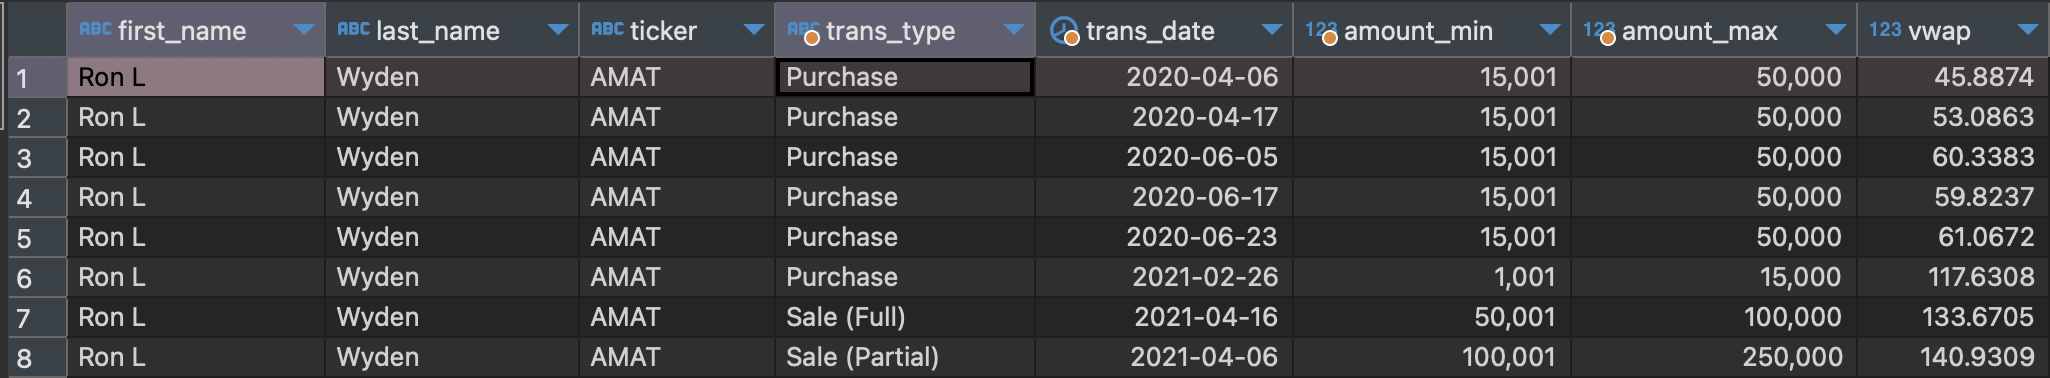
\includegraphics[width=1\textwidth]{imgs/RW-AMAT/RW-Trans.png}
  \caption{Transaction record of Senator Ron Wyden for ticker AMAT.}
  \label{fig:transaction_record}
\end{figure}

\begin{figure}[h]
  \centering
  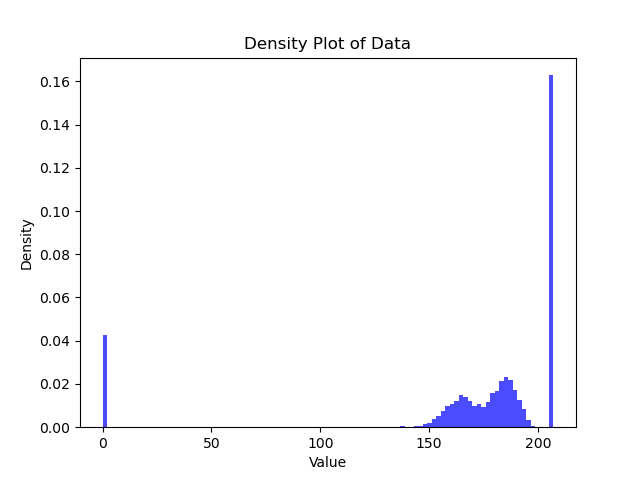
\includegraphics[width=1\textwidth]{imgs/RW-AMAT/RW-AMAT.png}
  \caption{Distribution of excess return of Senator Ron Wyden for ticker AMAT.}
  \label{fig:dist}
\end{figure}


\subsection{Results}

\begin{figure}[h!]
  \centering
  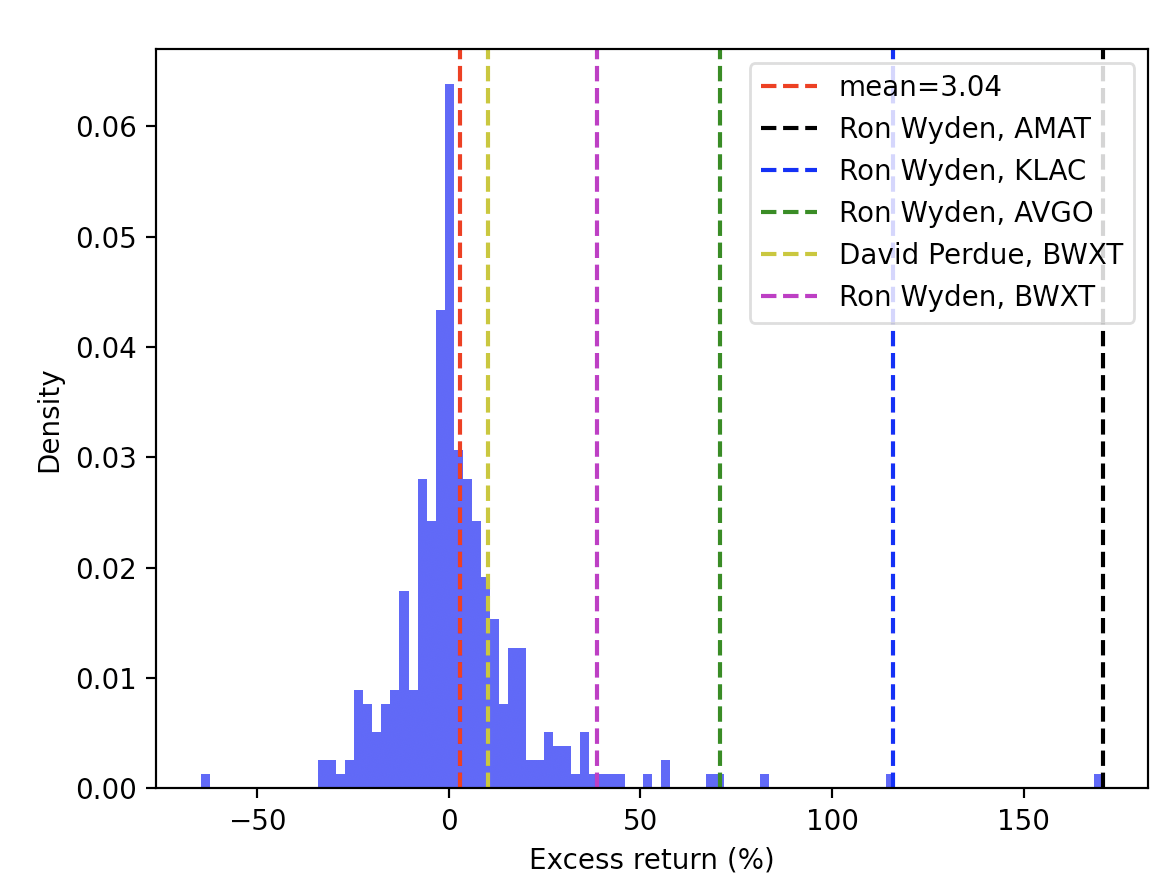
\includegraphics[width=1\textwidth]{imgs/ex-r/aggregate.png}
  \caption{Distribution of mean of each distribution of excess return for $333$ distinct pairs of (Senator, Ticker).}
  \label{fig:agg-ex-r}
\end{figure}

From the above explained approach, I collected mean of the distribution of excess return for $333$ distinct pairs of (Senator, Ticker). I found that the average excess return was $3.048\%$ with a standard deviation of $19.42$ (See Figure \ref{fig:agg-ex-r}). 

This analysis indicates that not all members of Congress are successful investors. Out of 333 (Senator, Ticker) pairs, only 173 recorded an excess return above $0\%$, which is just slightly over $50\%$ at $51.95\%$. This finding is consistent with \cite{eg13}, 
which concludes that the excess return of Congress members is not ``widespread''. However, \cite{eg13} found negative returns for almost all specifications for Senators between 2004-2008, 
while this analysis shows a mean excess return of $3.04\%$ and many outliers in the region above 0\%\footnote{In addition, the results provided in \cite{eg13} are at a fully aggregate level across legislators, so they do not capture any particular (Senator, Ticker) pairs with abnormally high returns.}. 
For example, there are $72$ (Senate, Ticker) pairs with a mean excess return above $5\%$, $31$ (Senate, Ticker) pairs above a mean excess return of $10\%$, and $8$ (Senate, Ticker) pairs with a mean excess return of more than 50\%.




% This result indicates that, on average, Congressmen earn a higher return on their investments compared to the general public, and the high standard deviation indicates that the return varies widely across Congressmen and investments.

\section{Anecdotes Revealing Congressional Insider Trading}

The analysis conducted 
in Section \ref{sec3} suggests that some elected officials may have been using their privileged access to information for personal financial gain. Here are some examples of financial transactions that may have been influenced by insider knowledge. I want to emphasize that the first two examples are already widely known through news and media as examples of congressional investment. This suggests that my algorithm is working well to identify abnormally high returns and suspicious investments that might be using privileged knowledge. Additionally, the last example has not been reported in the news or media, which suggests that my algorithm is also able to detect suspicious investments that are not widely known.

\subsection{Ron Wyden's Semiconductor Industry Investment}

Ron Wyden, a senator from Oregon, traded three semiconductor industry stocks, AMAT, KLAC, and AVGO, and obtained an estimated excess return of 170\%, 115\%, and 70\%, respectively (See Figure \ref{fig:agg-ex-r}). What is striking is that he purchased all three stocks on the same day, April 6, 2020, when the market was plummeting due to fears of the pandemic's impact on the economy. He then sold them all on the same day, April 6, 2021, after President Biden called for a \$50 billion boost to the US chips industry. As the chair of the Senate finance committee, it is reasonable to infer that Ron Wyden had prior knowledge of this issue before it became public.

\subsection{David Perdue's Investment in BWX Technologies Inc.}

David Perdue, a former senator from Georgia, obtained an estimated excess return of 10\% from his investment in BWX Technologies Inc., a company that supplies nuclear components to the US Navy (See Figure \ref{fig:agg-ex-r}). What is notable is that he made consecutive purchases of the stock that turned into sales after he was named chairman of the Senate Armed Services Subcommittee on Seapower on January 19, 2019.

\subsection{Ron L Wyden's Transaction on Constellation Brands Inc.}

In a transaction that was not widely reported in the media, Ron L Wyden, a senator from Oregon, sold his previously purchased shares of Constellation Brands Inc. (ticker: STZ), a producer and marketer of beer, wine, and spirits in the United States, after the US imposed tariffs on French and German wines in December 2020. This transaction resulted in an excess return of 38\%. As the chair of the Senate finance committee, which has jurisdiction over reciprocal trade agreements, it is possible that this transaction was based on privileged knowledge. Therefore, committee assignments may be strongly correlated with this transaction.

\section{Future directions}
So far is my current progress on my SYP. I briefly discussed this issue with Insong and decided to start with the most cited paper, Eggers (2013), which shows that Congressional investment is not as widespread as the public believes.

I collected my own data and conducted my own analysis to check whether congressmen actually enjoy excess returns above risk-free federal rates. As many media and news articles have cited, since the report only contains the min-max range of dollar amounts, they have had a hard time estimating how much excess returns they are enjoying and whether there are other transactions that could be reasonably suspected as insider trading.

I adopted a random sampling approach and I think I got quite satisfactory results. However, I would like to hear more from you about current analysis. Please feel free to come up with any questions or comments on the analysis so far.

As a next step, I would like to find a set of features that are more highly correlated with insider trading. It's hard to tell whether it's really insider trading or not, so I would like to set some threshold that I can accept as insider trading and see how the high-ranking feature sets diverge between those two groups. I think I can make a predictive model that predicts transacted tickers based on senator-specific predictors, such as their representing state, committee assignment, and previous transactions. Then, I can rank the features sorted by how helpful they've been in predicting the outcome. I don't have any specific model or method in mind yet, but I will generally incorporate some ML literature used in medical science for interpretability. Please feel free to cite or refer me to the articles that would be helpful.

In addition, I have to decide on features that could be used as my predictors for trading. I would like to wisely and strategically choose those feature sets because if I go too much toward unstructured data as my predictors, I'll run out of time and fail to make a successful SYP. I want to get some recommendations about which features will be useful and must be included based on your own hunch.

At this stage, I don't have any theory that explains a causal DAG that could explain this insider trading. I don't know whether this kind of paper can be evolve as a heavily theory-driven paper, and it would be better to focus on hypothesis testing to prove certain theories. Therefore I would like to more broadly incorporate any suggestions on what kind of narratives I can search for as a future direction.



\bibliography{biblo.bib}
\end{document}